\chapter{Introducción}\label{cap.introduccion}
El Trabajo Fin de Grado (TFG) descrito a continuación pertenece a un entorno educativo para la enseñanza de la programación de robots. En este capítulo se desarrollará el contexto en el que se sitúa este proyecto y la motivación que he llevado a su desarrollo. Es preciso comenzar con una explicación a grandes rasgos sobre qué es la robótica y sus aplicaciones en la sociedad.

La parte funcional más importante en la robótica viene suministrada por el software. Dentro del software podemos destacar diferentes elementos como los simuladores, las bibliotecas de código y los middlewares de robótica, los cuales serán descritos en la segunda sección del capítulo. En la tercera sección de este capítulo se describirá la situación actual de la robótica en el panorama educativo y en el entorno de JdeRobot-Academy, en el cual está desarrollado este TFG. La intención principal de su desarrollo es extender este entorno docente con nuevos ejercicios que representen un problema en la robótica. En cuanto al desarrollo de un sistema robótico, hay numerosas cuestiones a las que enfrentarse y solucionar. A la mayoría de estos problemas se enfrenta y soluciona el entorno docente y se oculta al estudiante, para que se pueda centrar en los algoritmos que dotarán vida al robot.

\section{Robótica}
A lo largo de la historia, la ciencia y la tecnología han sido utilizadas por el hombre para facilitarle la vida. Para ello, ha ideado, desarrollado y construido herramientas y máquinas empleándolas para reducir su carga de trabajo. En este entorno se desarrolla la robótica, que es la rama de la tecnología basada en la utilización de la informática para el diseño y desarrollo de sistemas automáticos que faciliten la vida al ser humano e, incluso, llegar a sustituirle en algunas tareas determinadas. La robótica incluye conceptos de disciplinas diversas, como la física, las matemáticas, la electrónica, la mecánica, la inteligencia artificial, la ingeniería de control, etc. Gracias a todas estas disciplinas involucradas unidas convenientemente se pueden diseñas máquinas que ejecuten comportamientos autónomos según el propósito para el que han sido desarrolladas. Estas máquinas autónomas se denominan "Robots".

El término "Robot" fue concebido por Isaac Asimov en 1950. Desde entonces estos sistemas autónomos han experimentado un crecimiento exponencial en cuanto a complejidad, versatilidad, autonomía y, sobre todo, en su incorporación a una gran diversidad de ámbitos. Los sistemas operados por el ser humano comienzan a incorporar un sistema de control específico programable que permiten el desarrollo de tareas repetitivas o con un gran riesgo para las personas, englobando tareas básicas y de difícil realización, hasta la actualidad, en la cual existe un gran marco de ejemplos en los que se integran la robótica y multitud de campos y tareas. Los robots comerciales e industriales realizan las tareas de una manera más exacta o más barata que las personas. También son utilizados en trabajos peligrosos, sucios tediosos para el ser humano. Gracias a esto, se trata de un campo en crecimiento constante.

\begin{figure}[H]
	\begin{center}
		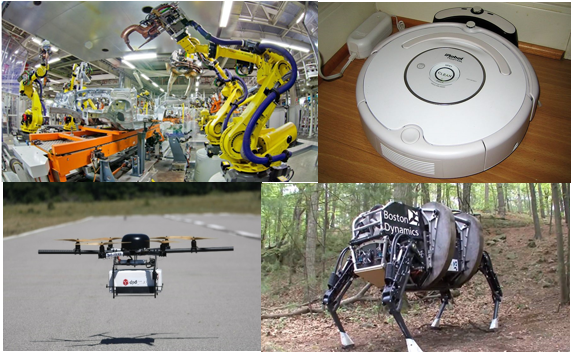
\includegraphics[width=0.8\textwidth]{figures/robots.png}
		\caption{Robots modernos}
		\label{fig.robots}
	\end{center}
\end{figure}

Ya se ha comentado la importancia de los robots en la actualidad en el aspecto industrial, pero tal el crecimiento que está experimentando la robótica que está comenzando a cobrar una gran importancia en aspectos menos especializados como el entorno doméstico. Cabe destacar el desarrollo de robots para facilitar la vida al ser humano, un ejemplo está ilustrado en la Figura 1.1. Las aspiradoras robóticas (Roomba, Dyson, Xiami, ...) han tenido un éxito rotundo en la realización de una actividad doméstica necesaria para la vida del ser humano. Otro éxito de la robótica en la actualidad es el desarrollo de coches autónomos. Este hecho se ha conseguido paulatinamente mediante la incorporación de tecnología cada vez más sofisticada a los automóviles. En este aspecto cabe destacar los módulos de aparcamiento automático, el park assist o los asistentes de conducción autónoma (autopiloto Tesla), o los prototipos de coches autónomos (Apple o Google). Otro ámbito en el que la robótica ha sido introducida es el militar, donde se han incorporado robots de rescate o para la desactivación de bombas. En la medicina se ha desarrollado el robot DaVinci, que permite operar desde cualquier parte del mundo con una precisión mayor a la humana. En el ámbito de la logística Amazon ha desarrollado una flota de robots de almacén que consiguen trasladar los pedidos a lo largo de sus almacenes. Tal es el punto de crecimiento de la robótica que se están desarrollando robots con "comportamientos inteligentes" como el robot Asimo de Honda (Figura 1.2) que pueden interactuar con humanos, ya sea como asistente para el hombre o con fines experimentales como la locomoción bípeda.

\begin{figure}[h]
	\centering
	\begin{minipage}[h]{.48\linewidth}
		\centering
		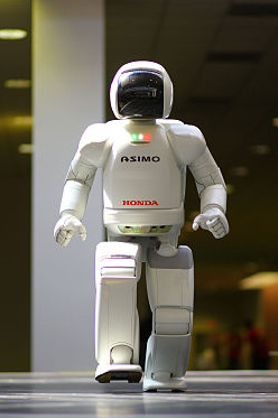
\includegraphics[width=.5\linewidth, height=7cm]{figures/asimo.png}
		\captionof{figure}{Robot Ásimo}
		\label{fig:asimo}
	\end{minipage}
	\begin{minipage}[h]{.48\linewidth}
		\centering
		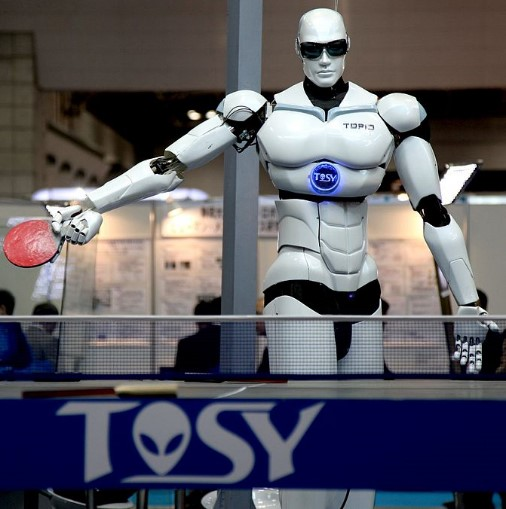
\includegraphics[width=.7\linewidth, height=7cm]{figures/topio.jpg}
		\captionof{figure}{Robot TOPIO}
		\label{fig:topio}
	\end{minipage}
\end{figure}

Los ámbitos en los que se puede aplicar la robótica es tan extenso como la imaginación de las personas dedicas a su creación, gracias a esto ámbitos en los que sólo podríamos imaginar automatizadas ahora son operadas totalmente con robots con resultados superiores a los de cualquier humano, como la agricultura de precisión mediante drones con análisis de imágenes térmicas y multiespectral para aumentar el rendimiento de las explotaciones agrícolas o el control de los productos industriales mediante el procesado de imágenes de la producción o la automatización de aplicaciones anestésicas de bajo nivel e, incluso, competiciones deportivas de robots.

Debido al gran potencial que tiene esta rama de la ciencia cobra una gran importancia la necesidad de dominarla. Gracias a ella ganaremos en comodidad, economía e, incluso, saludo. Es importante advertir de la importancia de la robótica en el futuro, ya que será la llave que abrirá la puerta a la humanidad hacia un mundo más seguro y sencillo mediante la automatización.

\section{Software Robótico}
Para que los robots puedan ser controlados de una manera eficaz el comportamiento del software que los controla debe ser robusto. Para ello se divide en distintas capas (\textit{drivers}, \textit{middleware} y aplicaciones), cuya arquitectura será distinta según su aplicación final.

Debido al gran desarrollo de la robótica, los robots actuales ya no precisan del control del ser humano para su funcionamiento, en la actualidad tienen comportamientos autónomos que les permiten realizar las tareas sin la mediación de terceros. Esto es posible gracias al minucioso desarrollo del software que compone los sistemas complejos del robot, algo parecido a una inteligencia autónoma. El desarrollo del software robótico parte de ciertas tareas o requisitos como son los circuitos de retroalimentación, control, búsqueda de caminos, localización o filtrado de datos entre otras muchas.

En los últimos años se han creado una gran cantidad de plataformas de desarrollo de software para las aplicaciones robóticas, también llamados /textit{middleware} robóticos. Los simuladores son otra parte importante para el desarrollo de software robótico ya que permiten realizar pruebas y depurar los fallos para programar una versión funcional del robot antes de ser fabricado. Esto supone un gran ahorro en costes. Estos componentes son vitales para generar el conjunto de comandos que componen la funcionalidad del robot, por ello entraremos en detalle en el siguiente apartado. Por último, las bibliotecas son necesarias para guardar los comandos que componen el funcionamiento del robot.

\subsection{Middlewares robóticos}
Los \textit{middleware} robóticos pueden definirse como entornos o \textit{frameworks} para el desarrollo de software pare robots. Se trata de software que conecta aplicaciones o componentes software para soportar aplicaciones complejas y distribuidas. Para controlar los sensores y actuadores de los robots estos entornos incluyen \textit{drivers}, arquitectura software para las aplicaciones que se van a crear, bloques de funcionalidad robótica ya resuelta, además de simuladores, visualizadores... Por ello al \textit{middleware} se le suele conocer como "pegamento para software". Una de las tareas del \textit{middleware} es conectar el hardware, ya sea real o simulado, con la aplicación desarrollada. El \textit{middleware} más extendido en el mundo es ROS.

	\textbf{Robot Operating System (ROS)\footnote{\url{http://www.ros.org/}}}

Se trata de una plataforma de software libre para el desarrollo software de robots que proporciona la funcionalidad de un sistema operativo en un clúster heterogéneo como el control de dispositivos de bajo nivel, mecanismos de intercambio de mensajes entre procesos y la abstracción del hardware, necesarios para el desarrollo de la robótica. Aunque el \textit{framework} ROS se desarrolló para los sistemas UNIX, se ha adaptado para ser soportado en otros sistemas operativos como Fedora, Debian, Windows, Mac OS X, Arch, Slackware, Gento u OpenSUSE, llegando a permitir las aplicaciones multiplataforma. Gracias a esto el \textit{framework} ROS se ha convertido en el más utilizado.

Existen otros \textit{framework} interesantes como:

	\textbf{Orocos}\footnote{\url{http://www.orocos.org/}}

Permitiendo el control avanzado de máquinas y robots en C++.

	\textbf{Orca}\footnote{\url{http://orca-robotics.sourceforge.net//}}

Está orientado a componentes por lo que permite el desarrollo de aplicaciones más complejas. Se tratta de un proyecto de software libre.

	\textbf{Urbi}\footnote{\url{https://github.com/urbiforge/urbi}}

Es un \textit{middleware} multiplataforma de código abierto en C++ que permite desarrollar aplicaciones en sistemas completos y complejos. Trabaja de forma conjunta con ROS.

	\textbf{JdeRobot}\footnote{\url{https://jderobot.org/}}

Plataforma de desarrollo de apicaciones robóticas y de visión artificial que incluye nodos programados con varios lenguajes de programación (Python o C++) compatible con \textit{middleware} de comunicaciones como ICE o ROS.

\subsection{Simuladores robóticos}
Debido al gran coste que supone la fabricación del hardware del robot es preciso depurar los posibles errores que contenga el código, así como el funcionamiento del hardware antes de su fabricación. Por ello debe probarse el código en un simulador orientado al tipo de aplicación que estemos desarrollando. Gracias a los simuladores es posible probar este código sin tener que fabricar previamente el hardware. De esta manera cualquier mal funcionamiento del código del robot puede ser solventado evitando la rotura del hardware. Algunos de los simuladores más utilizados son:

	\textbf{Gazebo}\footnote{\url{http://gazebosim.org/}}

Se trata del simulador 3D de código abierto más extendido. Funciona bajo la licencia Apache 2.0 y tienen gran importancia su motor de renderizado avanzado, sus motores de física y su soporte para \textit{plugins} de robot y sensores, además de su amplio catálogo de robots con sus sensores y actuadores. Otro hecho importante es su soporte para ROS lo que permite probar el código real del robot n el simulador.

	\textbf{Stage}\footnote{\url{http://wiki.ros.org/stage}}

Es un simulador en dos dimensiones, integrable con ROS, que permite simular numerosos robots simultáneamente.

	\textbf{Webots}\footnote{\url{https://www.cyberbotics.com/}}

Simulador de róbotica avanzada en el que se pueden desarrollar modelos propios y su física, escribir sus conroladores y hacer simulaciones a gran velocidad. Un ejemplo es su soporte para el humanoide Nao.

\subsection{Diseñadores Gráficos}
A la hora de introducir los modelos de los robots desarrollados en el simulador, así como un mundo simulado para comprobar la adaptación del mismo al medio, es necesario el uso de software de diseño gráfico. Este software permite la creación del modelo del robot e introducirla en el simulador. Gracias a esto se pueden ahorrar una gran cantidad de costes a la hora de desarrollar robots debido a que cualquier fallo estructural puede ser solventado antes incluso de la fabricación del prototipo. Algunos de los diseñadores gráficos más utilizados son:

	\textbf{SketchUp}\footnote{\url{https://www.sketchup.com/}}

Se trata de un programa de diseño gráfico y modelado en tres dimensiones basado en caras. Su principal característica es la realización de diseños en 3D de manera sencilla. Además incluye una extensa galería llamada 3D Warehouse que incluye esquemas de objetos, texturas e imágenes descargables. Este sofware de diseño es multiplataforma y de pago.

	\textbf{Blender}\footnote{\url{https://www.blender.org/}}

Es una programa de diseño gráfico dedicado especialmente al modelado, iluminación, renderizado, animación y creación de gráficos tridimensionales. También dispone de composición digital utilizand la técnica procesal de nodos, edición de vídeo, escultura (incluyendo topología dinámica) y pintura digital. También puede utilizarse para desarrollo de videojuegos dado que consta de una motor de juegos interno. Inicialmente fue distribuido de manera gratuita pero sin el código fuente, con un manual de uso, aunque posteriormente pasó a ser de software libre. Blender es multiplataforma con soporte para GNU/Linux, Windows, Mac OS X, Android, Solaris, FreeBSD e IRIX.

\subsection{Bibliotecas}
En el desarrollo de software deben abordarse un gran abanico de problemas clásicas, básicas y específicas para cada aplicación. Esta tarea es muy tediosa si hay que abordarla desde cero y requeriría un gran tiempo enfrentarse a ellas. Para evitar la repetición de problemas a la hora de desarrollar una aplicación, existen bibliotecas de código. Estas bibliotecas ofrecen conjuntos de implementaciones de código que permiten solucionar de manera directa ciertos problemas contenidos en su código. Esto permite al programador ahorrar una gran cantidad de tiempo para solucionar problemas que ya han sido solucionados anteriormente. Las bibliotecas pueden vincularse a un programa o a otra biblioteca en distintos puntos del desarrollo (bibliotecas estáticas) o durante la ejecución del programa (bibliotecas dinámicas). Algunas bibliotecas utilizadas en robótica son:

	\textbf{OpenCV}\footnote{\url{http://opencv.org/}}

Se trata de una biblioteca de código abierto que aborda problemas de visión artificial. Originalmente fue desarrollada por Intel y escrita en C++. En la actualidad contiene de interfaces en C++, Python, Java y MATLAB, además dispone de más de quinientas funciones que abarcan áreas de la visión artificial como reconocimiento de objetos y facial, calibración de cámaras y visión robótica y estéreo. Open CV es multiplataforma  y existen versiones para GNU/Linux, Mac OS X, Windows y Android.

	\textbf{OpenCV}\footnote{\url{http://pointclouds.org/}}

Es una librería utilizada para el procesamiento digital de imágenes RGBD mediante el tratamiento de nubes de puntos 3D. Entre sus numerosos algoritmos de última generación, se tratan problemas como filtrado, reconstrucción de superficies, ajuste de modelos, segmentación y estimación de características. Para simplificar el desarrollo, PCL se divide en bibliotecas de código  más pequeñas que pueden ser compiladas por separado. También es multiplataforma con soporte para Linux, Mac OS X, Windows y Android.

\section{Docencia en robótica}
La robótica con fines educativos está adquiriendo una gran importancia en la actualidad en la enseñanza preuniversitaria. Esto es debido a que su aprendizaje está disponible para estudiantes de cualquier nivel, el único requisito para estudiar robótico es la motivación por el desarrollo de aplicaciones. La robótica en el campo de la docencia cobra una gran importancia al ser una ciencia multidisciplinar, ya que incluye campos multidisciplinares como electrónica, informática, mecánica, física, ... Gracias a ello el estudiante adquiere una gran variedad de conocimiento de todas estas áreas. Además, proporciona una nueva visión del universo que le rodea, aprendiendo a distinguir los problemas y tomar una decisión al respecto.
En docencia primaria y secundaria se intenta despertar el interés del estudiante por la robótica, con la transformación de asignaturas teóricas tradicionales en asignaturas más prácticas e interactivas, ya que la robótica permite la recreación de problemas que les rodean y a través de los cuales pueden utilizar su creatividad y plasmar los conceptos teóricos que han adquirido.
En los centros de enseñanza primaria y secundaria se imparte robótica mediante plataformas físicas como los robots LEGO (Mindstorms, RCX, NXT, Evo, WeDo), placas Arduino, los kits de SolidWorks, etc.

\subsection{Docencias en la universidad}
En la docencia universitaria se imparte la robótica en distinto Grados y Postgrados en las escuelas de ingeniería. En España, se puede cursar la docencia robótica en el "Grado en Ingeniería Robótica" de la Universidad de Alicante, en los Grados de "Electrónica industrial y automática" o "Ingeniería Electrónica, Robótica y Mecatrónica" en distintas universidades, además de grados que están en desarrollo como el "Grado en Ingeniería Robótica Software" que imparte la Universidad Rey Juan Carlos desde el mes de Septiembre. Sin embargo, la docencia en robótica se reserva, mayoritariamente, para los Postgrados, dado que se trata una ciencia muy especializada. Existen varios Másteres destacados en cuanto a la docencia de robótica como el "Máster de Visión Artificial", el "Máster Universitario en Ingeniería Mecatrónica", o el "Máster Universitario en Automática y Robótica".
Dentro del ámbito internacional pueden encontrarse distintas universidades orientadas a robótica como el MIT, Carnegie Mellon University, Standford o Geordia Institute of Technology. También existen asociaciones prestigiosas como ACM (Association for Computing and Machinery) y la IEEE-CS (IEEE Computer Society) que ven la robótica como una ciencia imprescindible en estudios de ingeniería, informática y sistemas inteligentes.
En cuanto a la propia Universidad Rey Juan Carlos, cuenta con la plataforma docente JdeRobot, que consta de un entorno académico para la docencia de robótica llamado JdeRobot-Academy. Este entorno educativo se ha utilizado con éxito en distintas asignaturas como "Visión en Robótica" del Máster de Visión Artificial o en la asignatura Robótica del Grado de Ingeniería Telemática. Del mismo modo se han impartido talleres de aprendizaje para todos los públicos docentes, desde profesores de secundaria y primaria hasta estudiantes de secundaria pasando por trabajadores de distintas empresas. También se han impartido cursos de programación de drones para estudiantes universitarios.

\subsection{Entorno docente JdeRobot-Academy}
Los \textit{middleware} robóticos empleado para el desarrollo de este TFG son ROS y JdeRobot, que incluye el entorno académico JdeRobot-Academy\footnote{\url{https://jderobot.org/JdeRobot-Academy}}. Con este trabajo se ha pretendido extender sus posibilidades de aprendizaje, ampliándolo con dos nuevos ejercicios.
Los ejes en los que se apoya JdeRobot-Academy son:
\begin{enumerate}[label=\alph*)]
	\item Lenguaje Python (por su sencillez y potencia),
	\item simulador Gazebo (con distintos modelos de robot, tales como drones, formula1, brazos, aspiradoras, etc.), y
	\item foco en el algoritmo en vez de en el middleware, ocultando al estudiante los detalles de la infraestructura.
\end{enumerate}

El entorno JdeRobot-Academy cuenta con elenco de prácticas que abordan distintos problemas clásicos de la robótica. Para cada práctica se dispone de un componente académico que resuelve tareas auxiliares como la conexión con sensores y actuadores necesarios, la temporización o la interfaz gráfica y aloja el código del algoritmo del estudiante. De esta manera el estudiante se puede centrar en la solución del ejercicio exclusivamente. Cada nodo académico está formado por una parte específica oculta y el algoritmo con la lógica del robot del estudiante que se rellena en un fichero plantilla.

Debido a esta estructura, pueden distinguirse distintas capas en la composición de la práctica. La capa de nivel más bajo se le facilita al estudiante que sólo se centra en la capa superior donde se aloja la lógica del robot. Aunque esta capa más baja le viene dada al estudiante, es necesaria su implementación para poder dar solución a la práctica. En este aspecto se incluyen las conexiones de los sensores actuadores del robot, la interfaz gráfica, la temporización, el desarrollo del modelo del robot y un escenario que lo contenga, los plugins del modelo, los \textit{drivers} del mismo y la comunicación entre el simulador y el componente académico de alto nivel. Todo esto puede apreciarse en la Figura 1.4:

\begin{figure}[H]
  \begin{center}
    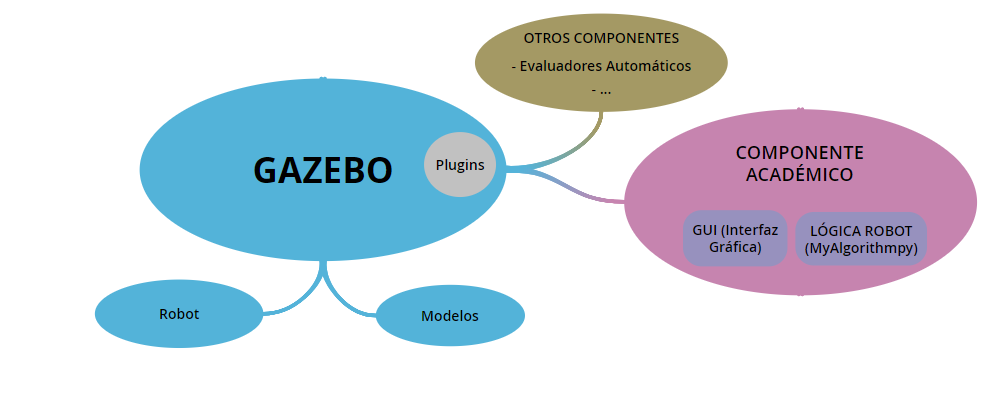
\includegraphics[width=0.9\linewidth]{figures/estructura_jde.png}
		\caption{Estructura de una práctica en JdeRobot-Academy}
		\label{fig.estructura}
		\end{center}
\end{figure}

Como se ha descrito anteriormente, en la Figura 1.4 se puede apreciar que la arquitectura software de las prácticas académicas facilita el desarrollo de las mismas por parte de los alumnos de manera que sólo se concentran en el desarrollo del algoritmo con la lógica del robot. El componente académico es el encargado de cargar en el simulador el código desarrollado por el alumno desde el fichero \textit{MyAlgorithm.py} y visualizar trazas que ayuden a la depuración del código como las imágenes procesadas, datos del láser o imágenes de la cámara integrada, dependiendo de la práctica.

El entorno usual para la realización de las prácticas es el simulador Gazebo, aunque las prácticas se han desarrollado de manera que puedan ser soportadas por robots reales sin realizar ninguna modificación, con los correspondientes drivers del robot. Gracias a esto, el código puede ser probado en robots reales. El sistema operativo base sobre el que se han desarrollado las prácticas es Linux dado que presenta una interfaz más sencilla a la hora de programar, por ello Linux cuenta con toda la infraestructura de las prácticas. 
Aunque en la actualidad se está terminando el entorno JdeRobot-Academy-Web en el que las prácticas docentes están almacenadas en un servidor y se puede acceder a ellas mediante el navegador. De esta manera se convierte al entorno JdeRobot en multiplataforma dotándolo de mayor accesibilidad. Esto es gracias al desarrollo de la interfaz web de Gazebo para la simulación, a la plataforma Jupyter (ver 3.6) que, mediante sus cuadernillos, han permitido trasladar las prácticas de JdeRobot-Academy al entorno docente JdeRobot-Academy-Web y al empleo de Dockers para dotar el entorno de un soporte multiplataforma.

Algunas de las prácticas que componen la plataforma son los siguientes:

\hspace{0.4\linewidth}
\textit{Follow Line}

\begin{figure}[H]
  \begin{center}
    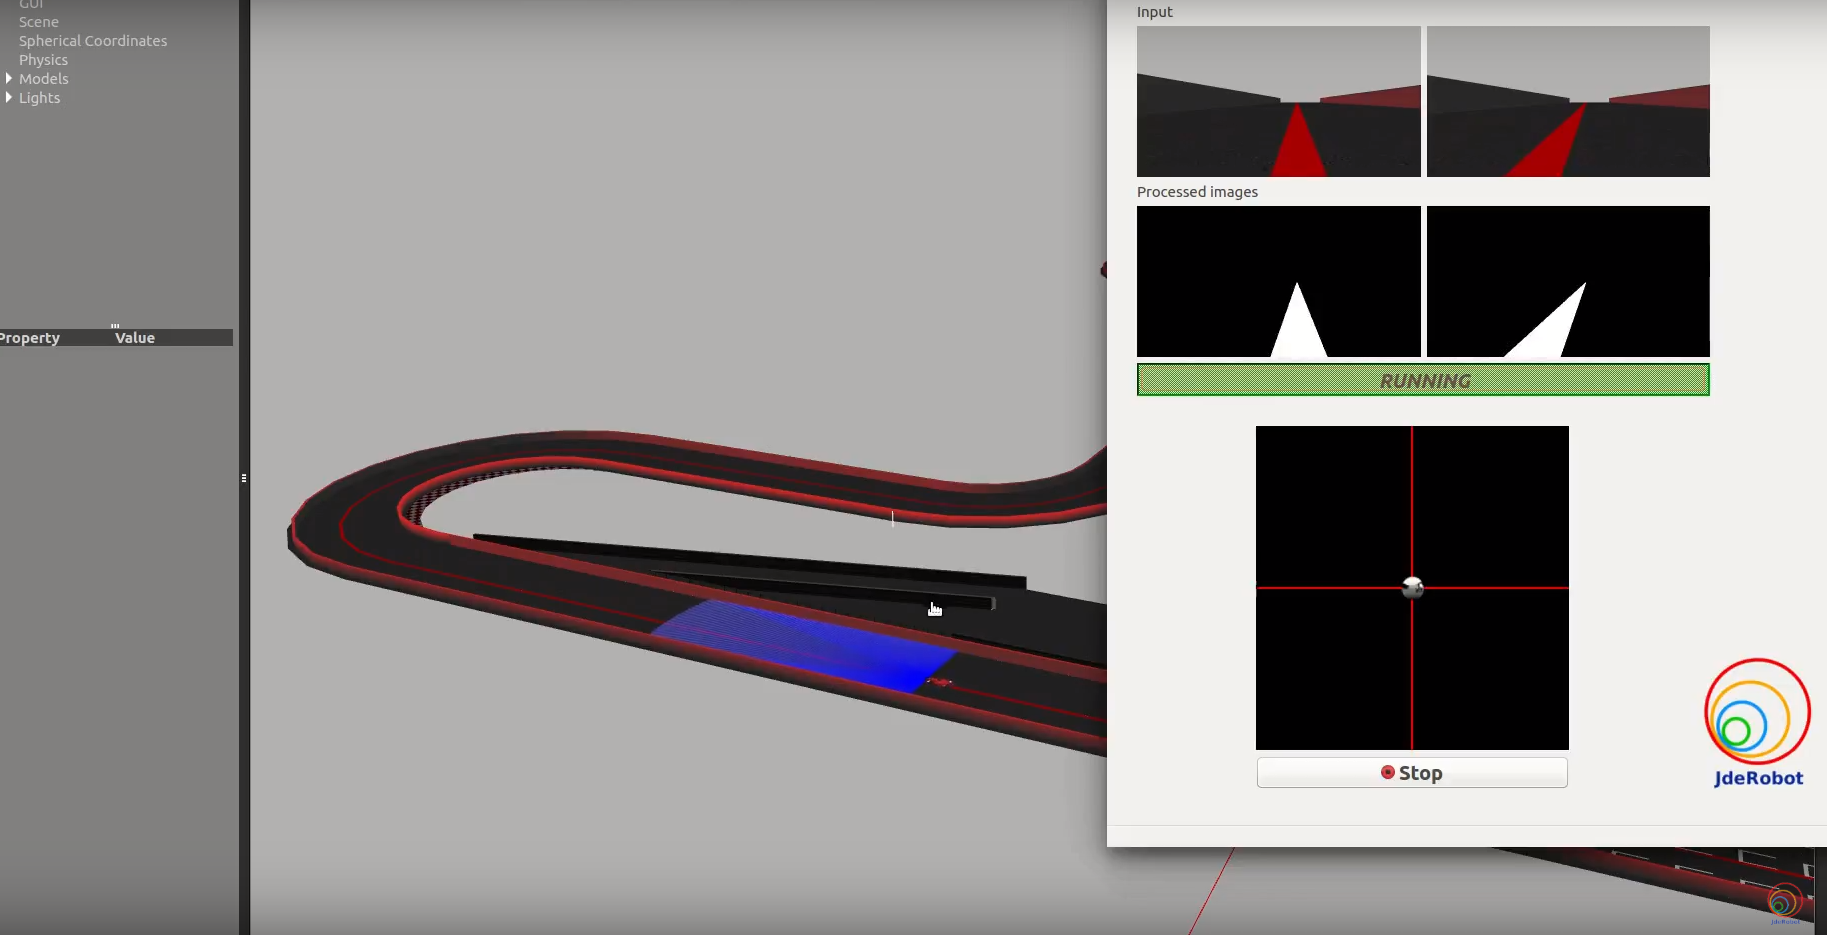
\includegraphics[width=0.95\textwidth]{figures/followline.png}
		\caption{Follow Line}
		\label{fig.followline}
		\end{center}
\end{figure}

Este ejercicio \textit{Follow Line} (Figura 1.5) trata de un robot coche Fórmula1 que consta de una cámara en su parte frontal por la que recoge imágenes. En su código se deben recoger las imágenes y procesarlas de manera que filtre la línea roja del circuito y la siga hasta que complete el circuito por completo \footnote{\url{https://youtu.be/QGO9oaoBVoA}}.

\vspace{4cm}
\hspace{0.40\linewidth}
\textit{Vacuum Cleaner}

\begin{figure}[H]
  \begin{center}
    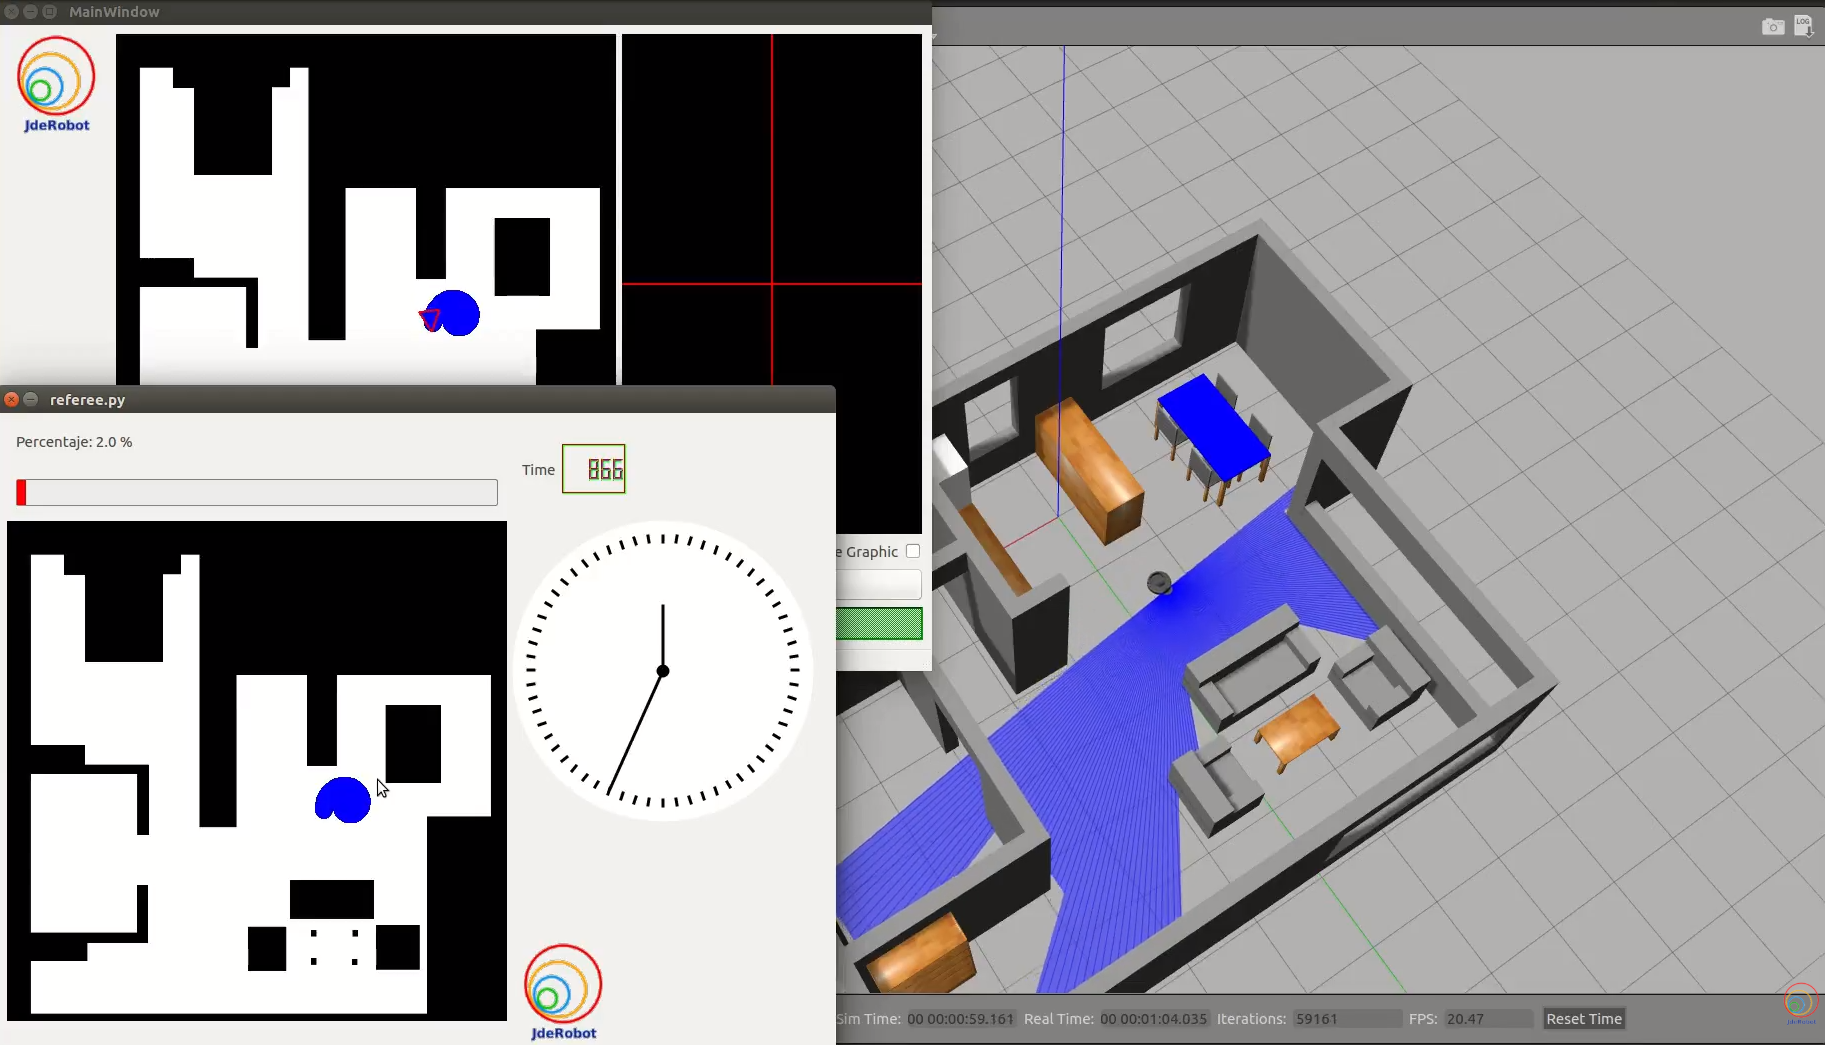
\includegraphics[width=0.50\linewidth, height=5cm]{figures/vacuumcleaner.png}
		\caption{Vacuum Cleaner}
		\label{fig.vacuumcleaner}
		\end{center}
\end{figure}

En este ejercicio \textit{Vacuum Cleaner} (Figura 1.6), el alumno debe recoger los datos del láser incluido en el modelo del robot aspiradora Roomba para que pase por el mayor área posible del escenario evitando la colisión con los obstáculos contenidos \footnote{\url{https://youtu.be/12muuY9JXLk}}.

\vspace{4cm}
\hspace{0.40\linewidth}
\textit{Visual Lander}

\begin{figure}[H]
  \begin{center}
    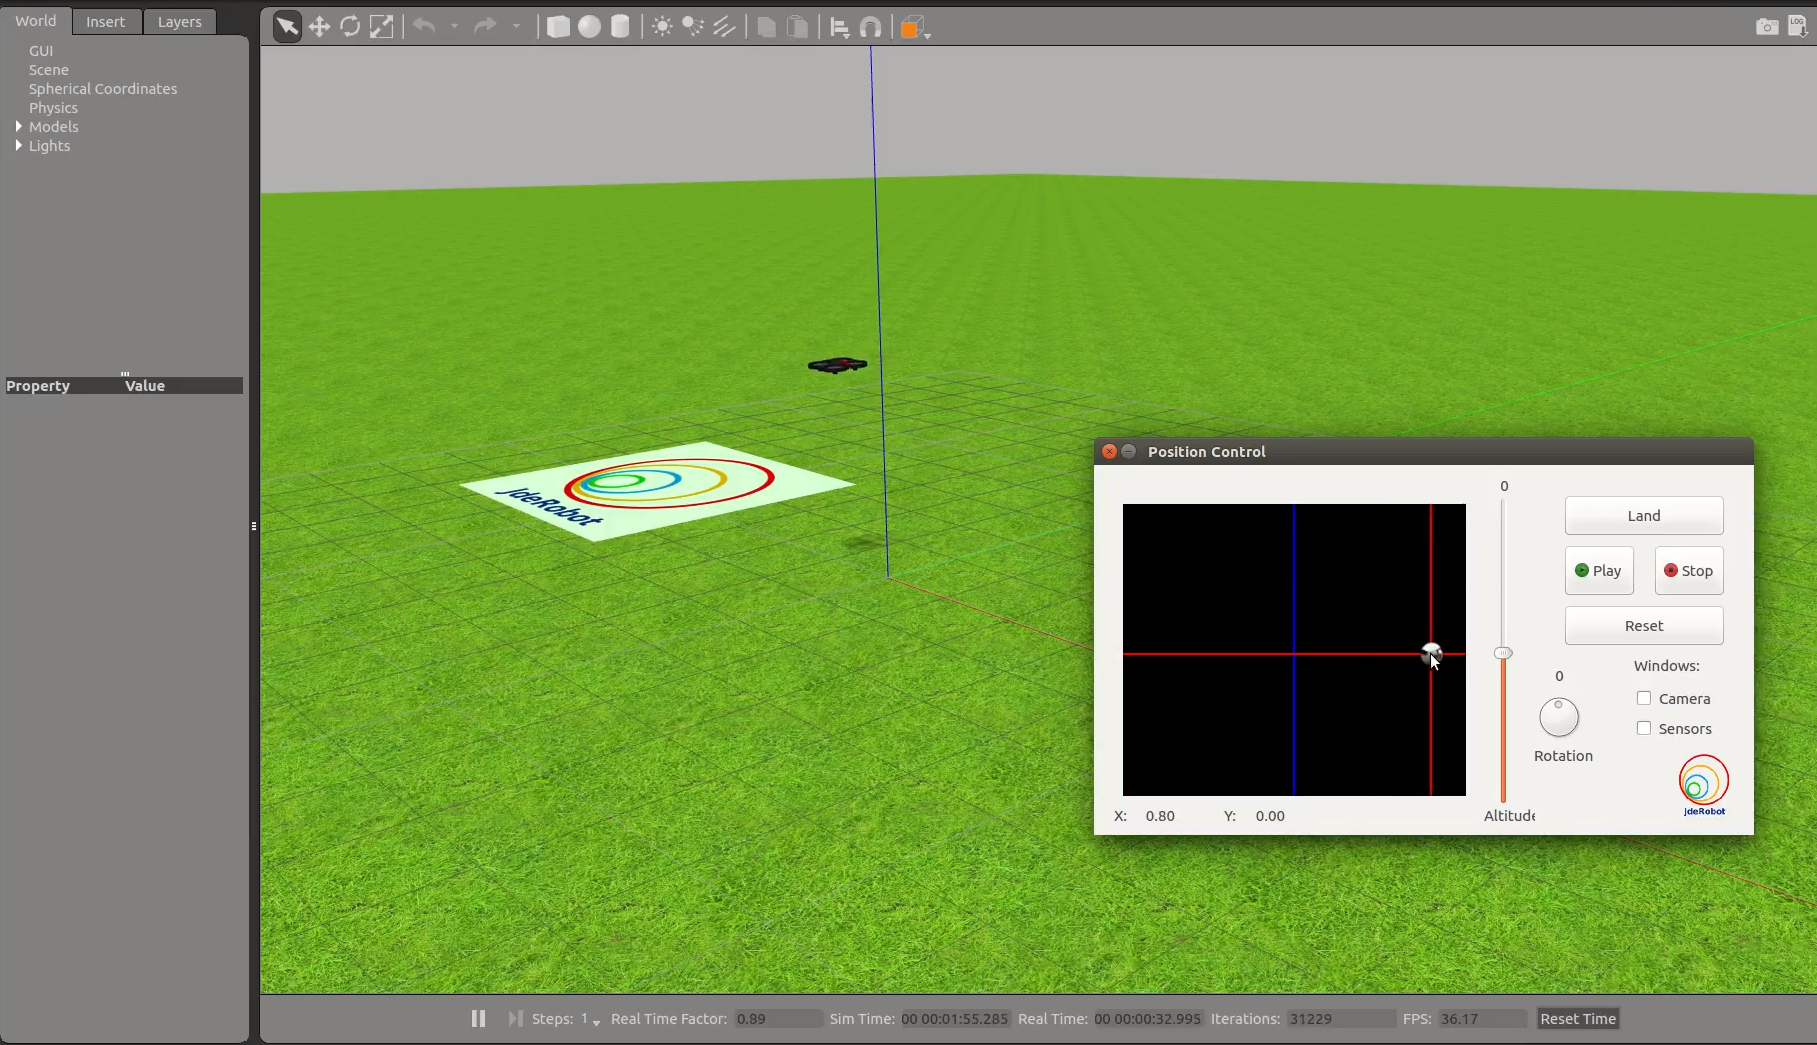
\includegraphics[width=0.50\linewidth, height=5cm]{figures/visuallander.png}
		\caption{Visual Lander}
		\label{fig.visual lander}
		\end{center}
\end{figure}

En este ejercicio \textit{Visual Lander} (Figura 1.7), el alumno deberá programar la lógica de un dron para que filtre las imágenes captadas por su cámara ventral y filtrarlas para distinguir una baliza y aterrizar controladamente sobre ella \footnote{\url{https://youtu.be/36pwaFYmDD0}}.

\vspace{4cm}
\hspace{0.40\linewidth}
\textit{Follow Turtlebot}

\begin{figure}[H]
  \begin{center}
    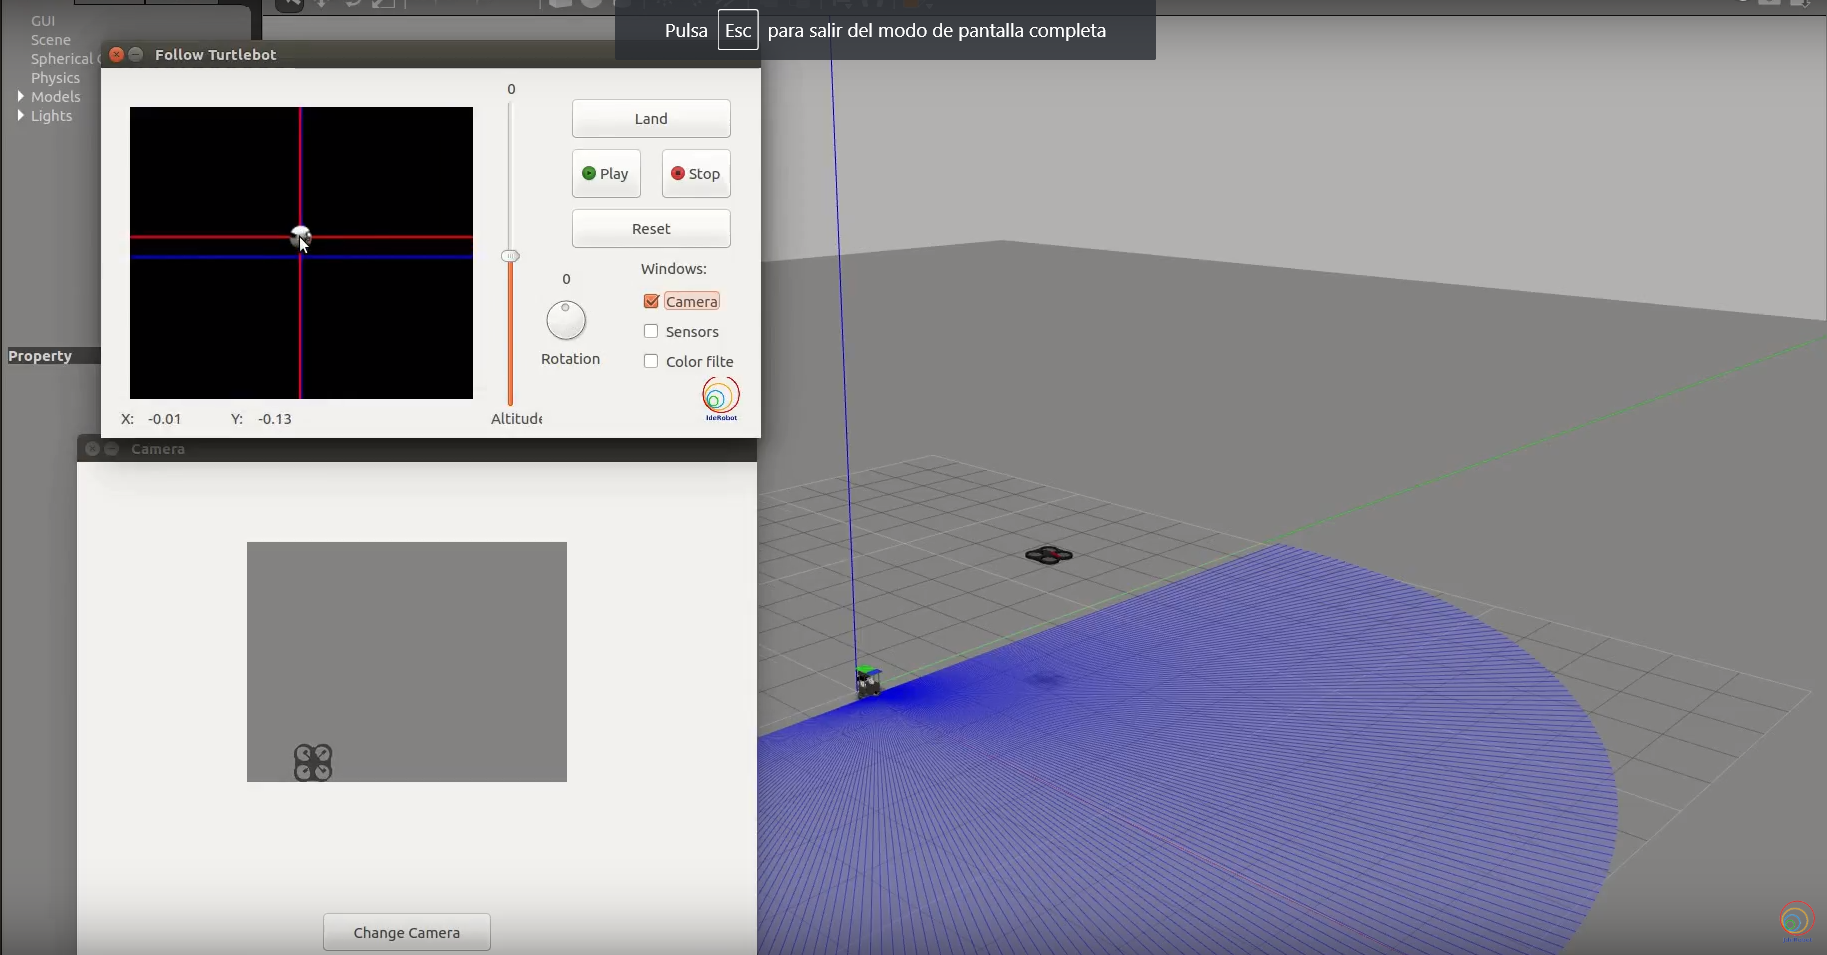
\includegraphics[width=0.50\linewidth, height=5cm]{figures/followturtlebot.png}
		\caption{Follow Turtlebot}
		\label{fig.followturtlebot}
		\end{center}
\end{figure}

Este ejercicio \textit{Follow Turtlebot} (Figura 1.8), consta de un escenario con un robot turtlebot teleoperado por el alumno y un dron. El código del algoritmo deberá dotar la inteligencia necesaria al dron para recoger las imágenes captadas por la cámara ventral del dron y filtrarlas para reconocer la baliza que lleva el turtlebot en su parte superior. Una vez reconocida debe dotar al dron de movimientos para seguirlo \footnote{\url{https://youtu.be/uehDVlBzpmU}}.

\vspace{7cm}
\hspace{0.35\linewidth}
\textit{Drone-Cat-Mouse}

\begin{figure}[H]
  \begin{center}
    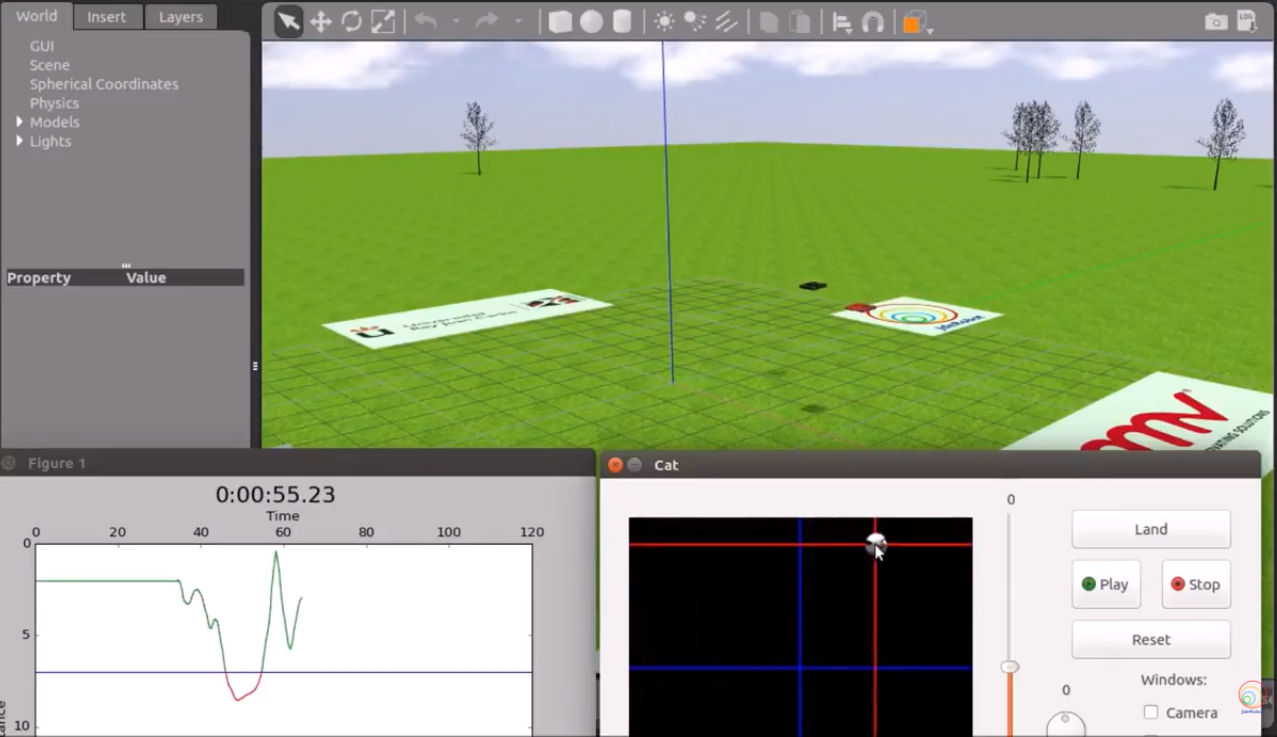
\includegraphics[width=0.95\textwidth, height=7.2cm]{figures/dronecatmouse.png}
		\caption{Drone-Cat-Mouse}
		\label{fig.dronecatmouse}
		\end{center}
\end{figure}

\textit{Drone-Cat-Mouse} es una de las prácticas más complejas del entorno JdeRobot-Academy. En ella el alumno debe dotar de la lógica necesaria a un dron (dron negro) para recoger las imágenes captadas por su cámara y filtrarlas para encontrar a un dron rojo. Una vez reconocido el dron rojo debe dotar de movimiento al dron para perseguirlo dado que el dron rojo está en movimiento. El objetivo es que el dron negro se acerque los más posible al dron rojo pero sin colisionar con él emulando el juego Gato-Ratón\footnote{\url{https://www.youtube.com/watch?v=DYD9oPawhWg}}. Esta práctica se ha utilizado en las dos ediciones del campeonato \textit{Program-A-Robot}, la primera en la URJC y la segunda en las Jornadas Nacionales de Robótica. Se va a utilzar en la tercera edición que tendrá lugar en la conferencia internacional IROS\footnote{\url{https://www.iros2018.org/competitions}}.

\subsection{Ejercicios recientes}

El contexto imediato de este Trabajo de Fin de Grado consiste en una serie de ejercicios elaborados recientemente  para enriquecer el contenido del entorno JdeRobot-Academy.

Entre los ejercicios elaborados más actuales caben destacar el TFG de Irene López Rodríguez \textit{"Nuevas Prácticas en el Entorno Docente de Robótica JdeRobot-Academy"}\cite{tfg1} en el que se introdujeron dos prácticas nuevas llamadas Coche autónomo negociando un cruce y Aspiradora autónoma con autolocalización. El primer ejercicio, después llamado \textit{Car Joint} trata sobre un coche autónomo que realiza un cruce por el que circulan coches. Para ello el coche debe filtrar las imágenes para reconocer una señal de Stop, así como los coches que circulan y las líneas de los carriles. Cuando no detecte ningún coche circulando debe tomar la intersección y escoger el carril correcto. La segunda práctica es similar a la práctica \textit{Vacuum Cleaner} pero consta del mapa con el escenario y sensor de posición, de manera que la aspiradora debe saber en qué lugar del escenario se encuentra y no repetir áreas ya limpiadas.

Otro TFG destacado en este aspecto es el de Vanessa Fernández Martínez \textit{{“Nuevas Prácticas en el Entorno Docente de Robótica JdeRobot-Academy”}}\cite{tfg2}, en el cual se añadieron dos prácticas nuevas llamadas Aspiradora Autónoma o \textit{Vacuum Cleaner} y Aparcamiento Automático, además de mejorar la práctica Tele Taxi con nuevos modelos, un mejor rendimiento del algoritmo GPP de navegación global y la inclusión de un evaluador automático capaz de medir el desempeño del algoritmo y proporcionar una nota. En cuanto al ejercicio desarrollado \textit{Vacuum Cleaner} ya ha sido comentado en el apartado anterior. La segunda práctica llamada \textit{Autopark} tiene como objetivo el aparcamiento de un coche autónomo mediante mediciones láser de los sensores frontales, laterales y posteriores.

También hay que mencionar el Trabajo de Fin de Grado desarrollado por Carlos Awadallah Estévez \textit{“Nuevas Prácticas Docentes de Robótica en el  Entorno JdeRobot-Academy”}\cite{tfg3}, en el cual se incorporan dos nuevas prácticas al entorno JdeRobot-Academy. La primera de ellas llamada \textit{Follow Face} trata de dar la lógica necesaria a una cámara pantilt de manera que procese las imágenes captadas por la cámara y reconozca la cara. Una vez hecho esto debe seguir el movimiento de la cara. La segunda práctica que se desarrolla en este TFG se llama \textit{Laser Loc} en la cual mediante mediciones de los sensores laser y un mapa con el escenario es capaz de realizar estimaciones de posición mediante movimiento y odometría.

Siguiendo con esta filosofía, el presente Trabajo de Fin de Grado aporta una práctica totalmente nueva al entorno JdeRobot-Academy y una optimización y mejora global de una práctica obsoleta incluyéndola en el entorno JdeRobot-Academy-Web.

\vspace{3cm}

El objetivo de este TFG es ampliar la variedad de prácticas que forman el entorno JdeRobot-Academy desarrollando nuevas prácticas y mejorando las exitentes para aumentar su versatilidad, además de aportar en el elenco de prácticas de JdeRobot-Academy-Web para acercar al entorno a dar soporte multiplataforma. En los próximos capítulos serán abordados los elementos necesarios para conseguir este objetivo. Comenzaremos con el Capítulo 2, en el que se concretarán los objetivos marcados, así como el punto de partida de este TFG y la metodología que ha sido empleada. En la Capítulo 3 se abordará la infraestructura utilizada para realizar el proyecto. En los Capítulos 4 y 5 explicaremos las prácticas que se han abordado en este TFG. Y, por último, en el Capítulo 6, se expondrán las conclusiones obtenidas, además de las posibles líneas de mejora futuras.

